% -*- coding: utf-8; ispell-dictionary: "french"; -*-

%----------------------------
% Chapter 1 - Fragment Scade
%----------------------------


Scade a été développé par le laboratoire Verimag à partir des travaux sur
le langage synchrone Lustre, puis repris par la société Esterel Technologies \cite{Estech}. On retrouve
ainsi les notions de Lustre dans le langage de Scade, un programme est découpé
en noeuds dont les entrées et sorties sont des \emph{flux de données}. Ces
noeuds sont les composants que nous voulons traduire. 
Les noeuds Scade considérés dans le cadre du projet \cercles  sont
soumis à quelques restrictions. En effet, il faut limiter le langage
utilisé, car certains éléments du langage sont spécifiques aux
langages synchrones et ne sont donc pas traduisibles en B.\\

% SECTION 1 : Présentation

\section{Architecture d'un composant Scade}

\paragraph{}
Scade étant un environnement de programmation par schémas-blocs, on
développe avec des "boîtes". Par exemple, un programme prenant en
entrées 3 entiers \texttt{b\_sup}, \texttt{b\_inf} et \texttt{z}, qui retourne un entier v égal
à:
\begin{itemize}
\item \texttt{z}, si \texttt{z} est compris entre \texttt{b\_inf} et \texttt{b\_sup}
\item \texttt{b\_inf}, si \texttt{z} est inférieur à \texttt{b\_inf}
\item \texttt{b\_sup}, si \texttt{z} est supérieur à \texttt{b\_sup}
\end{itemize}
Ce programme s'écrira de la façon suivante dans Scade. 

\begin{figure}[h]
\begin{center}
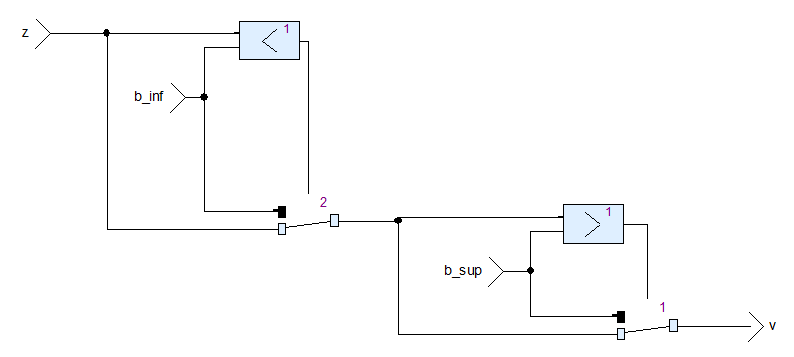
\includegraphics[scale=0.7]{1_bound.png}
\end{center}
\caption{Version graphique du noeud bound}
\end{figure}

La version textuelle de ce programme correspond au noeud \texttt{bound} suivant:

\begin{figure}[h]
\begin{center}
\begin{verbatim}
node bound (z: int; b_inf: int; b_sup: int) returns (v: int);
var
  a: int;
  c1: int;
  c2: int;
let
  a = if c1 then b_inf else z;
  v = if c2 then b_sup else a;
  c1 = z < b_inf;
  c2 = a > b_sup;
tel
\end{verbatim}
\end{center}
\caption{Version tectuelle}
\end{figure}

\paragraph{}
Au niveau des types de données utilisées, on pourra manipuler
des entiers, réels et booléens. On pourra également manipuler des
tableaux de ces types. En revanche, les types définis par
l'utilisateur tels que les types enregistrement ne seront pas gérés
par le traducteur.\\
Le comportement du noeud est ensuite défini par une liste d'équations,
dont l'ordre n'a pas d'importance. Ces équations sont de la forme:
\begin{verbatim}
left_part = expr;
\end{verbatim}
Où \texttt{left\_part} désigne une variable locale ou une sortie du composant, et expr
est une expression portant sur une ou plusieurs variables locales ou entrées.

\paragraph{}
Les expressions disponibles sont toutes les expressions arithmétiques
(\texttt{+, -, /, *, mod}), les expressions relationnelles (\texttt{<, >, <=, >=, =, <>})
et logiques (\texttt{and, or, xor, not}). Sont également disponibles les opérations sur les tableaux, telles que
la définition, l'index, et la concaténation. Lors de la génération
textuelle du noeud, Scade \emph{atomise} l'ensemble des opérations et
introduit des variables locales qui correspondent aux fils du
noeud. Pour ces opérations, la forme des équations sera donc toujours
semblable, on aura une seule variable à gauche de l'équation, et à
droite, on aura un opérateur appliqué à un ensemble de variables:

\texttt{v = op$_{base}$(x$_1$, ..., x$_n$);}\\
Les expressions conditionelles sont également possibles:

\texttt{v = if c then x$_1$ else x$_2$;}\\
avec \texttt{c}, \texttt{x$_1$} et \texttt{x$_2$} des variables. 

Enfin, on peut évidemment faire des appels à d'autres
noeuds, pour mettre en pratique la notion de composant
réutilisable. Les équations correspondantes peuvent avoir plusieurs
variables dans la partie gauche de l'équation, car un noeud appelé
peut avoir plusieurs sorties.

\texttt{v$_1$, ..., v$_p$ = op$_{appel}$(x$_1$, ..., x$_n$);}



% SECTION 2 : Restrictions

\section{Le temps avec Scade}

Le temps est un élément primordial dans ces systèmes dits "réactifs", où
l'on manipule des flux de données. Le temps est discrétisé en instants,
et chaque instant correspond à 1 tic de l'horloge de base. A chaque
instant i, les équations du noeud sont résolues à partir du flux reçu
en entrée à cet instant, et produit le flux de sortie correspondant au
résultat au même instant.

\paragraph{Une horloge unique}
Avec les langages synchrones, on peut
synchroniser des instructions sur des horloges différentes. On utilise des
opérateurs spécifiques au temps pour synchroniser une instruction sur une
horloge spécifique. Pour assurer la bonne définition des noeuds dont les
instructions sont calculées sur des horloges différentes, il existe
une étape de calcul des horloges \cite{Pouzet}.
Cependant, dans le cadre de ce projet, nous n'utiliserons qu'une seule horloge,
celle de base. Toutes les équations sont résolues au même instant. 

\paragraph{L'opérateur fby}
Il y a un seul opérateur temporel qui reste utilisable, c'est
l'opérateur \texttt{fby}. Cet opérateur prend 3 arguments:
\begin{itemize}
\item une variable v
\item un délai
\item une initialisation
\end{itemize}
A l'instant i\footnote{On suppose que le premier instant est l'instant
0}, \texttt{fby} retourne la valeur de la variable v à
l'instant (i - délai). Dans le cas ou (i - délai) est négatif,
l'opérateur retourne la valeur initialisation.
Par exemple, on représente dans le tableau suivant la valeur de sortie
de l'opérateur \texttt{fby} en fonction de la valeur d'une variable
d'entrée \texttt{v}, avec une initilisation à 0, et un délai fixé à 1.

\begin{figure}[h]
\begin{center}
\begin{tabular}{ l || c | c | c | c }
\texttt{instant} & 0 & 1 & 2 & ... \\ \hline
\texttt{v} & 10 & 20 & 30 & ... \\
\texttt{z} & 0 & 10 & 20 & ... \\
\end{tabular}
\end{center}
\caption{\texttt{z = fby(v, 1, 0)}}
\end{figure}

Cet opérateur permet de donner un \emph{état} à un composant, les
calculs des équations étant alors dépendants de l'instant où ils sont
effectués.
Par la suite, on appellera cette construction un \emph{registre}.


\section{Contrats}

On peut définir des assertions dans un noeud afin de poser des
restrictions sur les valeurs d'entrée ou de sortie du composant. Avec
Scade, ces assertions sont possibles avec :
\begin{itemize}
\item \texttt{assume A: expr}, où \texttt{A} correspond à l'identifiant de la condition, et
\texttt{expr} un prédicat portant sur une entrée du noeud: une précondition.
\item \texttt{guarrantee G: expr}, où \texttt{G} est l'identifiant de la condition, et
\texttt{expr} un prédicat portant sur une sortie du noeud: une postcondition.
\end{itemize}
Ces assertions forment le contrat du composant, et seront
obligatoires sauf pour la restriction sur les booléen qui est triviale (la
valeur sera vraie ou fausse). Pour les entiers et les réels, on
indiquera des intervals de valeurs.\\

Par exemple, en reprenant le noeud \texttt{bound} précédent, on donne comme condition sur
les entrées qu'elles doivent être comprises entre -2000 et 2000 inclus. Si les
préconditions sont respectées, alors la sortie sera comprise entre -2000
et 2000 inclus:
\begin{figure}[h]
\begin{center}
\begin{verbatim}
node bound (z: int; b_inf: int; b_sup: int) returns (v: int);
var
  a: int;
  c1: int;
  c2: int;
let
  assume A_1 : b_inf <= 2000 and b_inf >= -2000;
  assume A_2 : b_sup <= 2000 and b_sup >= -2000;
  assume A_3 : z <= 2000 and z >= -2000;
  guarantee G_1 : v <= 2000 and v >= -2000;
  a = if c1 then b_inf else z;
  v = if c2 then b_sup else a;
  c1 = z < b_inf;
  c2 = a > b_sup;
tel
\end{verbatim}
\end{center}
\caption{Noeud bound avec contrat}
\end{figure}

